
\section{Frontend that we know}
\begin{frame}
  \frametitle{Frontend that we know}
Now we are going to talk about approaches used at today's systems. \newline

I use the example about the blog page:
\begin{itemize}
	\item Microservice which manage users, authentication etc.
	\item Microservice for articles (listing, creating, editing, etc.)
	\item Frontend is SPA/SPA like
\end{itemize}
\end{frame}


\subsection{Monolith}

\begin{frame}
	\frametitle{Monolith}
	It's important to understand something about structure of application.
	So, we have one big block of code:
	\begin{figure}
		\centering
		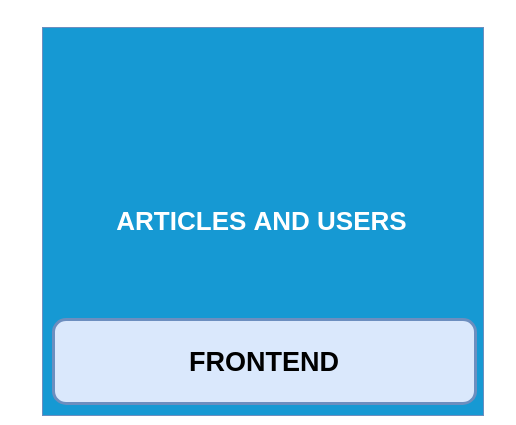
\includegraphics[width=0.6\linewidth]{pictures/monolit.png}		
		\label{fig:monolit}
	\end{figure}
\end{frame}

\begin{frame}
	\frametitle{Pros\&Cons}
	\begin{columns}[t]
		\column{0.5\linewidth}
			\textbf{\begin{center}
				+
			\end{center}}
		
		\begin{itemize}
			\item Everything at one place
			\item Probably - at one pull request we can add new feature 
			\item Deployed once with a frontend. We are sure that both layers work fine togeth
		\end{itemize}
		
		
		\column{0.5\linewidth}
			\textbf{\begin{center}
				--
			\end{center}}
		
		\begin{itemize}
			\item Scalability
			\item Complex inside
			\item A lot of legacy code can exist
		\end{itemize}
	
	\end{columns}
\end{frame}

\subsection{Monolith with REST}
\begin{frame}
\frametitle{Monolith with REST}
We(developers) like to have layers and separations. So a lot of systems have REST interface(or similar). We can work more parallel. Also, we have two smaller codebases.
\begin{figure}
	\centering
	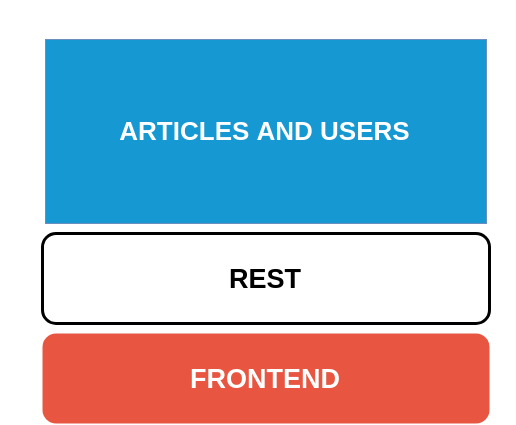
\includegraphics[width=0.55\linewidth]{pictures/monolit-and-rest.png}		
	\label{fig:monolith-rest}
\end{figure}
\end{frame}
\subsection{Microservices}

\begin{frame}
\frametitle{Microservices}
	\begin{figure}
		\centering
		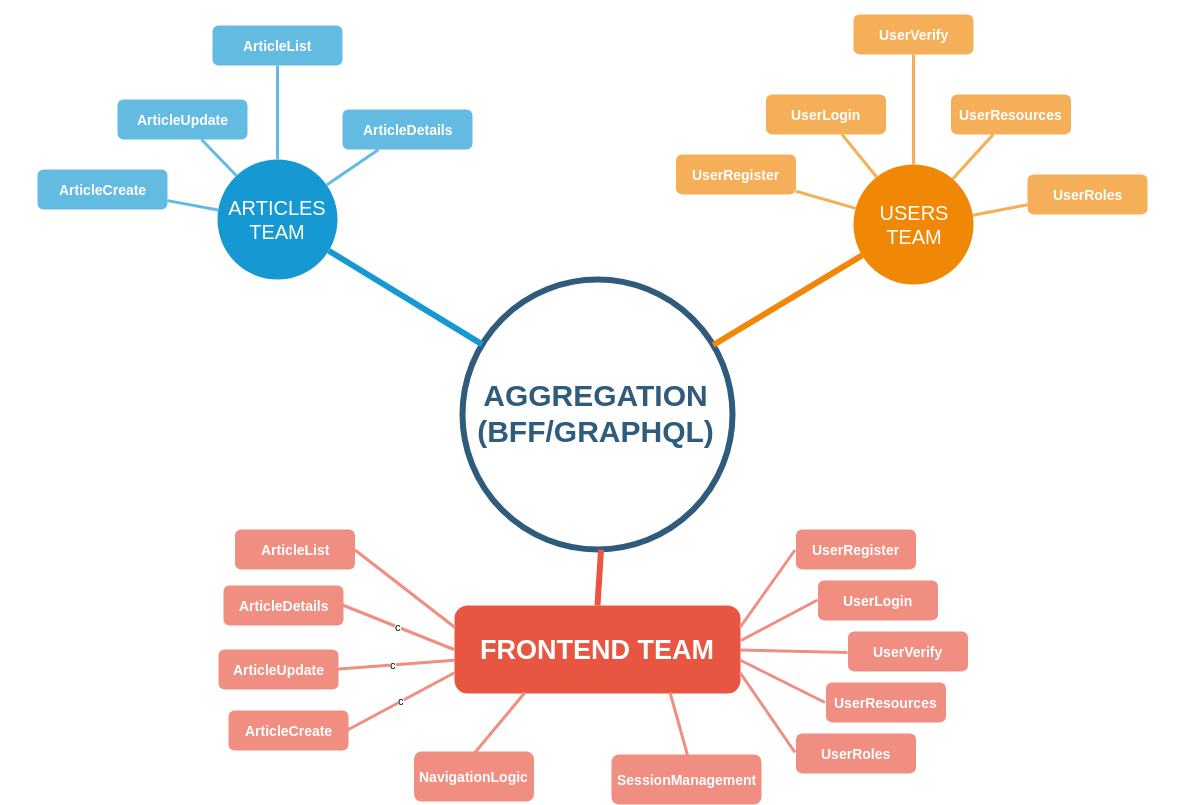
\includegraphics[width=0.8\linewidth]{pictures/microservices-knowledge.png}		
		\label{fig:microservices}
	\end{figure}
\end{frame}


